%% USPSC-Apendice.tex
% ---
% Inicia os apêndices
% ---

\begin{apendicesenv}
	% Imprime uma página indicando o início dos apêndices
	\partapendices
	\chapter{Additional tables of the textual differences found in all networks}\label{ap:textd}
In the following tables the counting of differences of textual features among the analyzed networks
are shown.
	These results are auxiliary for the discussion on Section~\ref{sec:tresults}.
\FloatBarrier
\begin{table}[h!]
\begin{center}
\caption{Counts of evidence of characters-related differences in the Erd\"os sectors in each of the analyzed networks.}
	\def\arraystretch{1.5}
\begin{tabular}{| l || c | c | c || c |}\hline
{\bf synset} & {\bf p.} & {\bf i.} & {\bf h} & {\bf peaks} \\\hline\hline
$\frac{spaces}{chars}$ & 2  & 0  & 8  & 2 \\
$\frac{punct}{chars-spaces}$ & 11  & 4  & 1  & 5 \\
$\frac{digits}{chars-spaces}$ & 9  & 7  & 2  & 10 \\\hline
$\frac{letters}{chars-spaces}$ & 0  & 0  & 3  & 0 \\
$\frac{vowels}{letters}$ & 0  & 1  & 1  & 1 \\
$\frac{uppercase}{letters}$ & 13  & 3  & 1  & 6 \\\hline
\end{tabular}
\begin{flushleft}
		Source: By the author.\
\end{flushleft}
\end{center}
\end{table}

\begin{table}[h!]
\begin{center}
\caption{Counts of evidence of token-related differences in the Erd\"os sectors in each of the analyzed networks.}
	\def\arraystretch{1.5}
\begin{tabular}{| l || c | c | c || c |}\hline
{\bf synset} & {\bf p.} & {\bf i.} & {\bf h} & {\bf peaks} \\\hline\hline
$\frac{knownw}{tokens}$ & 1  & 0  & 5  & 1 \\
$\frac{knownw \neq}{knownw}$ & 13  & 1  & 4  & 9 \\
$\frac{stopw}{knownw}$ & 0  & 0  & 14  & 2 \\
$\frac{punct}{tokens}$ & 10  & 3  & 1  & 3 \\
$\frac{contrac}{tokens}$ & 0  & 2  & 15  & 4 \\\hline
$\mu(\overline{tokens})$ & 0  & 1  & 2  & 1 \\
$\sigma(\overline{tokens})$ & 7  & 1  & 0  & 2 \\\hline
$\mu(\overline{knownw})$ & 0  & 0  & 2  & 0 \\
$\sigma(\overline{knownw})$ & 0  & 0  & 1  & 1 \\\hline
$\mu(\overline{knownw \neq})$ & 0  & 0  & 0  & 0 \\
$\sigma(\overline{knownw \neq})$ & 0  & 0  & 0  & 0 \\\hline
$\mu(\overline{stopw})$ & 0  & 0  & 0  & 0 \\
$\sigma(\overline{stopw})$ & 0  & 0  & 1  & 0 \\\hline
\end{tabular}
\begin{flushleft}
		Source: By the author.\
\end{flushleft}
\end{center}
\end{table}

\begin{table}[h!]
\begin{center}
\caption{Counts of evidence of sentence-related differences in the Erd\"os sectors in each of the analyzed networks.}
\begin{tabular}{| l || c | c | c || c |}\hline
{\bf synset} & {\bf p.} & {\bf i.} & {\bf h} & {\bf peaks} \\\hline\hline
$\mu_S(chars)$ & 9  & 3  & 1  & 6 \\
$\sigma_S(chars)$ & 11  & 6  & 1  & 9 \\\hline
$\mu_S(tokens)$ & 10  & 2  & 1  & 5 \\
$\sigma_S(tokens)$ & 9  & 7  & 1  & 9 \\\hline
$\mu_S(knownw)$ & 9  & 3  & 2  & 6 \\
$\sigma_S(knownw)$ & 11  & 5  & 2  & 8 \\\hline
$\mu_S(stopw)$ & 2  & 3  & 7  & 7 \\
$\sigma_S(stopw)$ & 6  & 7  & 4  & 10 \\\hline
$\mu_S(puncts)$ & 13  & 2  & 1  & 2 \\
$\sigma_S(puncts)$ & 7  & 8  & 1  & 8 \\\hline
\end{tabular}
\begin{flushleft}
		Source: Prepared by the authors.\
\end{flushleft}
\end{center}
\end{table}

\begin{table}[h!]
\begin{center}
\caption{Counts of evidence of message-related differences in the Erd\"os sectors in each of the analyzed networks.}
	\def\arraystretch{1.5}
\begin{tabular}{| l || c | c | c || c | c |}\hline
{\bf synset} & {\bf p.} & {\bf i.} & {\bf h} & {\bf peaks} & {\bf total} \\\hline\hline
$\mu_M(sents)$ & 4  & 7  & 1  & 9  & 16 \\
$\sigma_M(sents)$ & 5  & 7  & 2  & 11  & 15 \\\hline
$\mu_M(tokens)$ & 10  & 5  & 2  & 6  & 18 \\
$\sigma_M(tokens)$ & 8  & 8  & 2  & 9  & 18 \\\hline
$\mu_M(knownw)$ & 8  & 5  & 3  & 7  & 18 \\
$\sigma_M(knownw)$ & 10  & 5  & 3  & 9  & 18 \\\hline
$\mu_M(stopw)$ & 5  & 6  & 6  & 8  & 18 \\
$\sigma_M(stopw)$ & 7  & 6  & 3  & 11  & 18 \\\hline
$\mu_M(puncts)$ & 12  & 4  & 2  & 5  & 18 \\
$\sigma_M(puncts)$ & 8  & 9  & 1  & 10  & 18 \\\hline
$\mu_M(chars)$ & 10  & 5  & 2  & 6  & 18 \\
$\sigma_M(chars)$ & 9  & 7  & 2  & 8  & 18 \\\hline
\end{tabular}
\begin{flushleft}
		Source: Prepared by the authors.\
\end{flushleft}
\end{center}
\end{table}

\begin{table}[h!]
\begin{center}
\caption{Counts of evidence of differences related to POS tags in the Erd\"os sectors in each of the analyzed networks.}
\begin{tabular}{| l || c | c | c || c |}\hline
{\bf synset} & {\bf p.} & {\bf i.} & {\bf h} & {\bf peaks} \\\hline\hline
NOUN & 13  & 1  & 0  & 1 \\
X & 4  & 9  & 5  & 14 \\\hline
ADP & 0  & 1  & 4  & 1 \\
DET & 1  & 0  & 9  & 2 \\\hline
VERB & 0  & 0  & 6  & 1 \\\hline
ADJ & 1  & 2  & 6  & 2 \\
ADV & 0  & 0  & 17  & 1 \\\hline
PRT & 1  & 1  & 9  & 4 \\
PRON & 0  & 1  & 11  & 3 \\
NUM & 8  & 5  & 3  & 7 \\
CONJ & 2  & 6  & 4  & 8 \\\hline
\end{tabular}
\begin{flushleft}
		Source: By the author.\
\end{flushleft}
\end{center}
\end{table}

\begin{table}[h!]
\begin{center}
\caption{Counts of evidence of differences related to Wordnet POS tags in the Erd\"os sectors in each of the analyzed networks.}
\begin{tabular}{l || c | c | c || c}\hline
{\bf synset} & {\bf p.} & {\bf i.} & {\bf h} & {\bf peaks} \\\hline\hline
N & 8  & 1  & 0  & 1 \\
ADJ & 0  & 2  & 12  & 6 \\
VERB & 0  & 1  & 16  & 2 \\
ADV & 0  & 0  & 9  & 1 \\\hline\hline
POS & 0  & 0  & 3  & 1 \\
POS! & 0  & 1  & 0  & 1 \\\hline
\end{tabular}
\begin{flushleft}\footnotesize
		Source: By the author.\
\end{flushleft}
\end{center}
\end{table}

\begin{table}[h!]
\begin{center}
\caption{Counts of evidence of differences related to Wordnet noun synset characteristics in the Erd\"os sectors in each of the analyzed networks.}
\begin{tabular}{| l || c | c | c || c |}\hline
{\bf synset} & {\bf p.} & {\bf i.} & {\bf h} & {\bf peaks} \\\hline\hline
$\mu(min\,depth)$ & 0  & 0  & 0  & 0 \\
$\sigma(min\,depth)$ & 1  & 1  & 2  & 1 \\\hline
$\mu(max\,depth)$ & 0  & 0  & 0  & 0 \\
$\sigma(max\,depth)$ & 0  & 1  & 3  & 1 \\\hline
$\mu(holonyms)$ & 7  & 4  & 4  & 6 \\
$\sigma(holonyms)$ & 3  & 4  & 7  & 6 \\\hline
$\mu(meronyms)$ & 8  & 5  & 3  & 7 \\
$\sigma(meronyms)$ & 12  & 4  & 2  & 9 \\\hline
$\mu(domains)$ & 6  & 4  & 5  & 8 \\
$\sigma(domains)$ & 3  & 1  & 4  & 3 \\\hline
$\mu(lemmas)$ & 6  & 0  & 1  & 2 \\
$\sigma(lemmas)$ & 6  & 2  & 2  & 4 \\\hline
$\mu(hyponyms)$ & 1  & 6  & 6  & 9 \\
$\sigma(hyponyms)$ & 4  & 6  & 6  & 11 \\\hline
$\mu(hypernyms)$ & 0  & 0  & 0  & 0 \\
$\sigma(hypernyms)$ & 4  & 4  & 4  & 6 \\\hline
\end{tabular}
\begin{flushleft}
		Source: Prepared by the authors.\
\end{flushleft}
\end{center}
\end{table}

\begin{table}[h!]
\begin{center}
\caption{Counts of evidence of differences related to Wordnet adjective synset characteristics in the Erd\"os sectors in each of the analyzed networks.}
\begin{tabular}{| l || c | c | c || c |}\hline
{\bf synset} & {\bf p.} & {\bf i.} & {\bf h} & {\bf peaks} \\\hline\hline
$\mu(domains)$ & 2  & 6  & 8  & 10 \\
$\sigma(domains)$ & 2  & 4  & 5  & 7 \\\hline
$\mu(similar)$ & 1  & 0  & 7  & 4 \\
$\sigma(similar)$ & 4  & 0  & 5  & 3 \\\hline
$\mu(lemmas)$ & 1  & 2  & 1  & 2 \\
$\sigma(lemmas)$ & 6  & 3  & 4  & 6 \\\hline
\end{tabular}
\begin{flushleft}
		Source: By the author.\
\end{flushleft}
\end{center}
\end{table}

\begin{table}[h!]
\begin{center}
\caption{Counts of evidence of differences related to Wordnet verb synset characteristics in the Erd\"os sectors in each of the analyzed networks.}
\begin{tabular}{| l || c | c | c || c |}\hline
{\bf synset} & {\bf p.} & {\bf i.} & {\bf h} & {\bf peaks} \\\hline\hline
$\mu(min\,depth)$ & 2  & 1  & 1  & 3 \\
$\sigma(min\,depth)$ & 2  & 1  & 1  & 2 \\\hline
$\mu(max\,depth)$ & 2  & 1  & 0  & 1 \\
$\sigma(max\,depth)$ & 3  & 1  & 1  & 2 \\\hline
$\mu(domains)$ & 7  & 3  & 4  & 4 \\
$\sigma(domains)$ & 8  & 3  & 3  & 5 \\\hline
$\mu(verb\,groups)$ & 0  & 2  & 3  & 2 \\
$\sigma(verb\,groups)$ & 0  & 0  & 0  & 0 \\\hline
$\mu(lemmas)$ & 0  & 0  & 2  & 0 \\
$\sigma(lemmas)$ & 1  & 0  & 3  & 0 \\\hline
$\mu(entailments)$ & 7  & 1  & 7  & 3 \\
$\sigma(entailments)$ & 4  & 1  & 5  & 3 \\\hline
$\mu(hyponyms)$ & 1  & 2  & 6  & 3 \\
$\sigma(hyponyms)$ & 2  & 3  & 8  & 6 \\\hline
$\mu(hypernyms)$ & 2  & 2  & 0  & 2 \\
$\sigma(hypernyms)$ & 1  & 0  & 1  & 1 \\\hline
\end{tabular}
\begin{flushleft}
		Source: By the author.\
\end{flushleft}
\end{center}
\end{table}

\begin{table}[h!]
\begin{center}
\caption{Counts of evidence of differences related to Wordnet adverb synset characteristics in the Erd\"os sectors in each of the analyzed networks.}
\begin{tabular}{| l || c | c | c || c |}\hline
{\bf synset} & {\bf p.} & {\bf i.} & {\bf h} & {\bf peaks} \\\hline\hline
$\mu(domains)$ & 3  & 3  & 10  & 10 \\
$\sigma(domains)$ & 1  & 4  & 7  & 7 \\\hline
$\mu(lemmas)$ & 0  & 0  & 1  & 1 \\
$\sigma(lemmas)$ & 3  & 1  & 2  & 4 \\\hline
\end{tabular}
\begin{flushleft}
		Source: Prepared by the authors.\
\end{flushleft}
\end{center}
\end{table}


	\chapter{Definition of the terms of text-related measurements}\label{ap:textd}
	The following terms are used in Sections~\ref{sec:cha}-\ref{subsec:pc} and Appendix~\ref{ap:textd}.
	The measurements related to part-of-speech (POS) were defined directly at Tables~\ref{tab:pos} and~\ref{tab:wnpos}.
\begin{table}[h!]
\begin{center}
\caption{Definition of text-related measurement terms.}
	\def\arraystretch{1.5}
\begin{tabular}{l || c }\hline
{\bf term} & {\bf definition} \\\hline\hline
chars & characters \\
punct & punctuations \\
digits & numerical digits \\
letters & alphabetical letters \\
uppercase & uppercase letters \\\hline
knownw & known words \\
knownw $\neq$ & different known words \\
contrac & contractions \\
stopw & stopwords \\\hline
$\mu$ & mean \\
$\sigma$ & standard deviation \\\hline
$\overline{something}$ & the size of \emph{something} \\
	$\mu_S(something)$ & mean of sizes of sentences measured by counting \emph{something} \\
	$\sigma_S(something)$ & standard deviation of sentences measured by counting \emph{something} \\
	$\mu_M(something)$ & mean of sizes of messages measured by counting \emph{something} \\
	$\sigma_M(something)$ & standard deviation of messages measured by counting \emph{something} \\\hline
\end{tabular}
\begin{flushleft}\footnotesize
		Source: By the author.\
\end{flushleft}
\end{center}
\end{table}


	\chapter{Developments made in this research but not included elsewhere in this thesis}\label{ap:more}
In this appendix are gathered developments relevant for an important proposal of this research:
enabling the use of complex networks scientific knowledge by the participant of the social networks.
These developments are not included elsewhere in the thesis because we chose to present results
more closely related to physics in a simple fashion which is more suitable for a computational and applied physics doctorate thesis.
Most of the following contributions have received dedicated documentation,
reason why we next only summarize and cite the documents when they are available.
Another motivation for including this chapter is for obtaining an organization of these contributions
which are scattered in public webpages, repositories and private documents.
I understand that they have received dedication of many intellectuals
and furthermore are useful for future research.

\section{Continuous voting by approval and participation}\label{ap:vot}
In finding the adequate way to prioritize proposals, the Brazilian social participation community agreed about the measurement of two indexes,
one of approval and one of participation. Both practice and literature
was constantly handled by the experts involved, and the formalization
of such model and metrics and is very simple and seems novel.
Also, the relevance of this development is strengthened by the use of these indexes by the
Brazilian General Secretariat of the Republic to raise and prioritize
proposals about public health care in open processes.
This was achieved by means of the Dialoga Brasil federal platform~\cite{dialoga}.
A short report on these indexes and their use is on~\cite{dialogaAlg}
	(co-authorship by Ricardo Poppi).

	\section{Visualization of static networks}
	In Sections~\ref{sec:versinus0} and~\ref{sec:versinus1} we address a visualization method of networks through animations.
	We also made many static network visualizations which were important for our research.
	Many of these were made by testing software and programming libraries.
	We next exemplify such efforts by some of the most important realizations.

	\subsection{Static email network visualization using Networkx, Graphviz and a PHP web interface}\label{sec:autoRede}
	At the start of this research, we observed many networks derived from email lists
	by means of a web interface we wrote.
	In such web interface, which was accessed as a usual webpage through HTTP in a web browser, 
	the user could specify an email list, start and end messages and a window size (number of messages taken together to obtain the network).
	The interface then rendered graph visualizations and standard measures such as degree, strength, clustering coefficient, betweenness centrality, both as histograms and as mean and standard deviation.
	In the node-link diagrams, measurements were mapped to height, width and color of nodes and to link characteristics.
	There was also a very similar interface aimed at comparing networks.
	The software source code is available in~\cite{autoRede} and an example image is Figure~\ref{fig:autoRede}.
\begin{figure}[h!]
\begin{center}
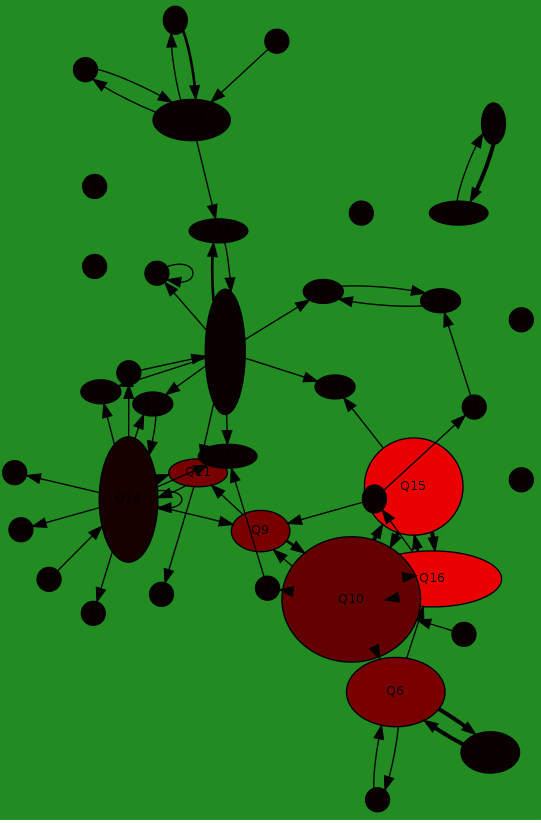
\includegraphics[scale=.25]{figs/autoRede_}
\caption{An example image rendered from the first online gadget made in this research for studying social networks.
	The app also delivered measurements, 2D plots and graph files (GML and GDF).
	For further information please see Section~\ref{sec:autoRede}}
\label{fig:autoRede}
\begin{flushleft}\footnotesize
Source: By the author.\
\end{flushleft}
\end{center}
\end{figure}
% email pelo app online

	\subsection{Static Facebook networks visualization using Gephi}\label{sec:gephi}
	Mainly in the years of 2013 and 2014, Facebook users retrieved their friendship networks through Netvizz software~\cite{netvizz}
	and donated them to our research.
	I also retrieved my friendship network (a number of times) 
	and friendship and interaction networks from Facebook groups I was a member, also using Netvizz.
	These networks were used for information collection and diffusion (explained in Section~\ref{sec:colDif}),
	taking measurements and visualization.
	The visualizations were achieved almost exclusively through the Gephi software~\cite{gephi}
	and is included in this appendix for being used a number of times by fellow researchers and artists.
	The most useful layout algorithm was Force Atlas 2~\cite{fa2} and an example of these images is Figure~\ref{fig:gephi}.

% \begin{figure}[h!]
% \begin{center}
% 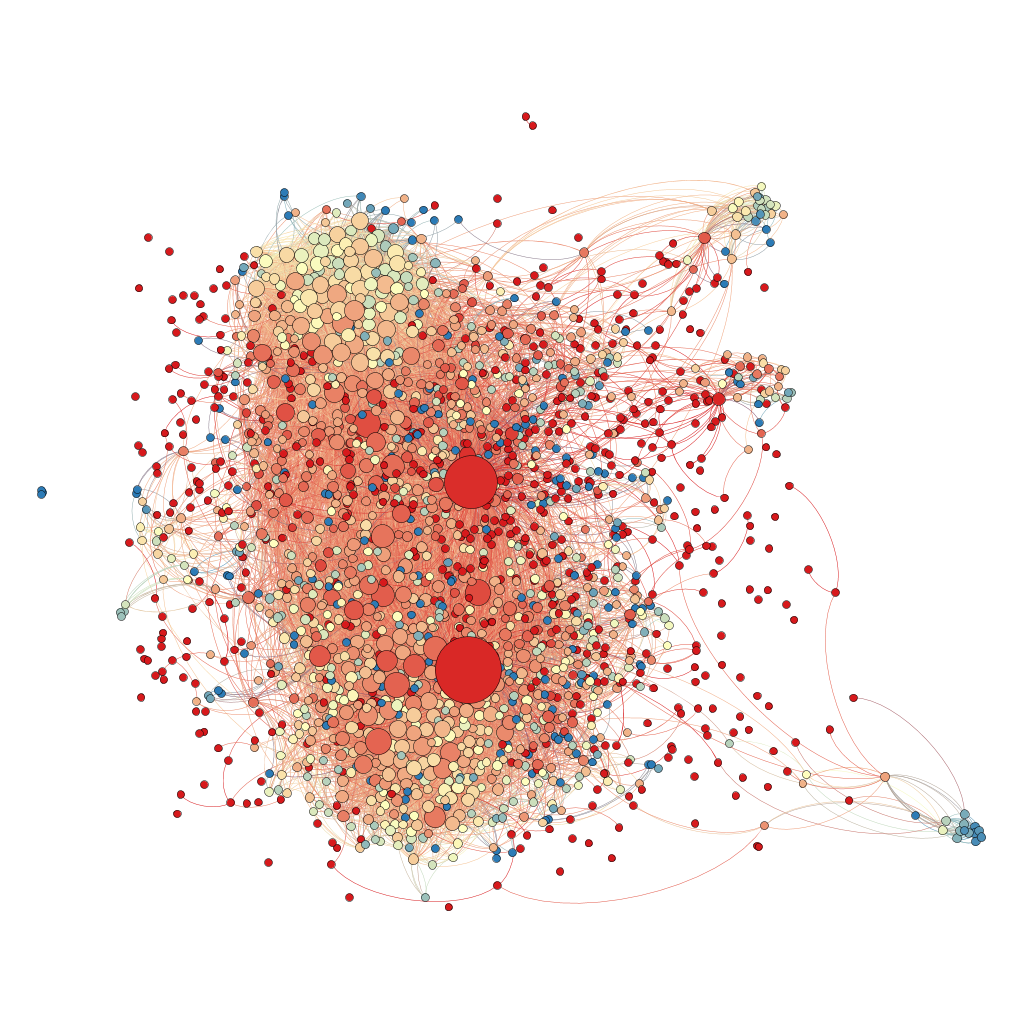
\includegraphics[scale=.25]{figs/Silicon}
% 	\caption{An example network image rendered from the Silicon Valley (Facebook) group using Gephi and the Force Atlas 2 layout algorithm.
% 	See Section~\ref{sec:gephi} for further information.}
% \label{fig:gephi}
% \begin{flushleft}\footnotesize
% Source: By the author.\
% \end{flushleft}
% \end{center}
% \end{figure}

\begin{figure}[!tbp]
	\centering
	    \subfloat[\footnotesize Without participant names.]{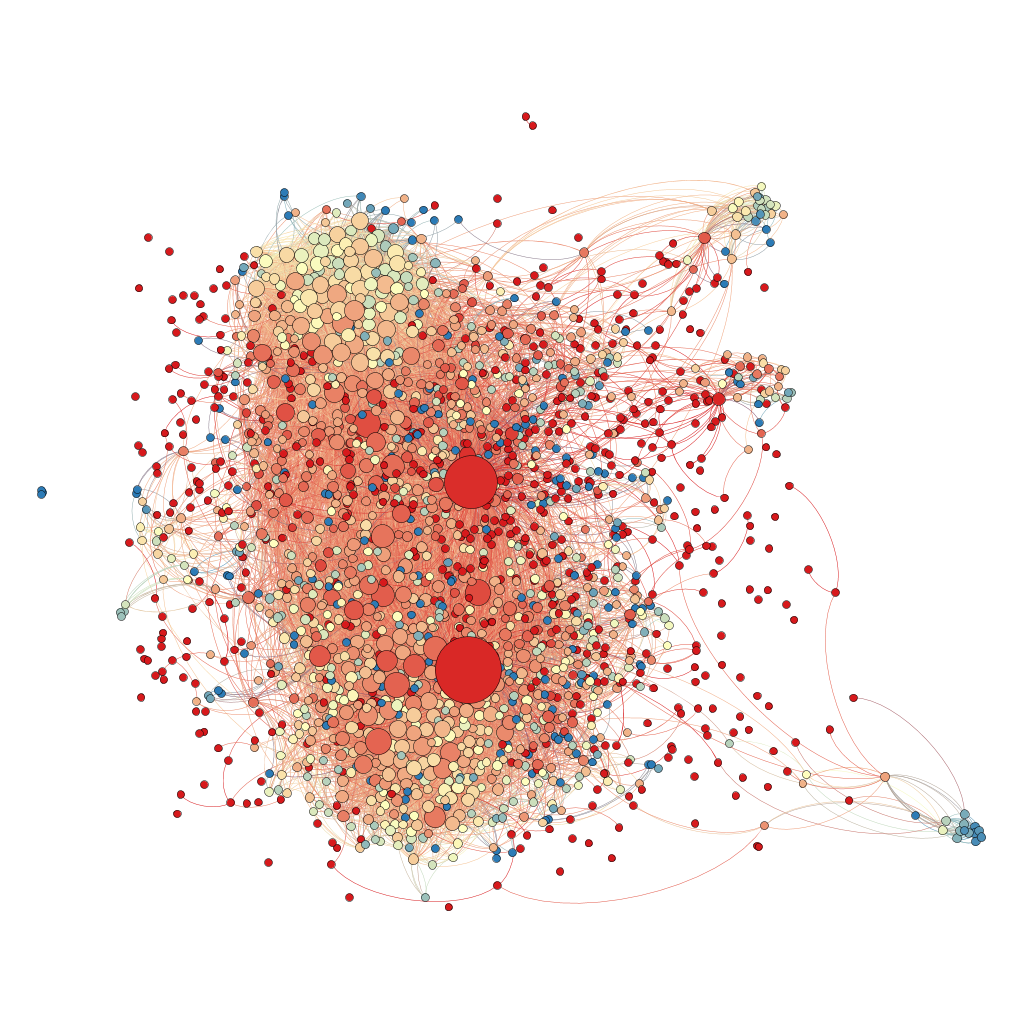
\includegraphics[width=0.45\textwidth]{figs/Silicon.png}\label{fig:f1}}
		\subfloat[\footnotesize With participant names.]{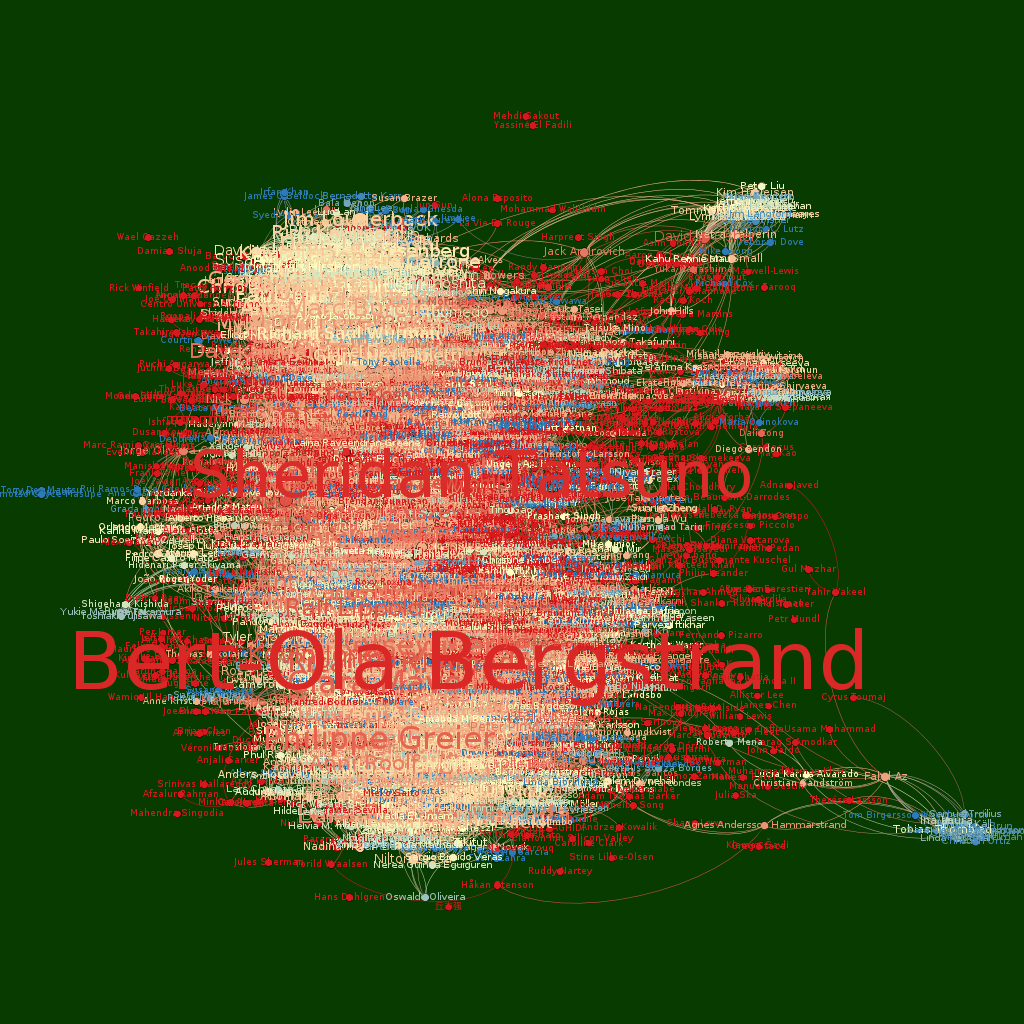
\includegraphics[width=0.45\textwidth]{figs/Silicon_nomes.png}\label{fig:f2}}
	\caption{An example network image rendered from the Silicon Valley (Facebook) group using Gephi and the Force Atlas 2 layout algorithm.
	See Section~\ref{sec:gephi} for further information.}\label{fig:gephi}
\begin{flushleft}\footnotesize
Source: By the author.\
\end{flushleft}
\end{figure}

	\subsection{Art on networks by Pedro Paulo Rocha}\label{sec:ppr}
	The static images rendered for the visualization of networks were at time also used for artistic elaborations.
	Apart from other artistic incidences reported in this appendix (such as in Sections~\ref{sec:govArt} and~\ref{sec:soundSkull})
	we present in Figure~\ref{fig:ppr} an example art from Pedro Paulo Rocha.
	More of his work that is derived from our network visualizations are gathered in an image gallery~\cite{pprGal}.
\begin{figure}[h!]
\begin{center}
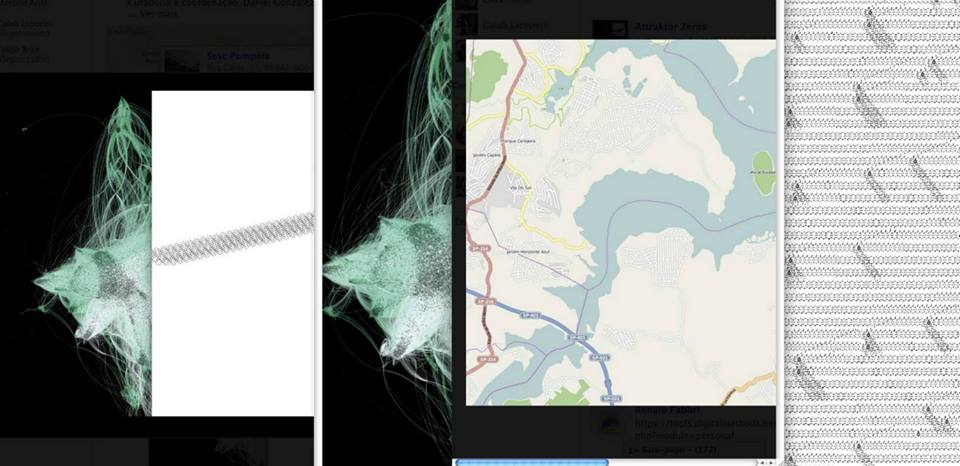
\includegraphics[scale=.45]{figs/ppr}
\caption{An example artistic image by Pedro Paulo Rocha and derived from our network visualizations.
	For further information see Section~\ref{sec:ppr}}
\label{fig:ppr}
\begin{flushleft}\footnotesize
Source: Provided by the artist Pedro Paulo Rocha. Image derived from other images by the author.\
\end{flushleft}
\end{center}
\end{figure}

\section{Mega networks: connecting many Facebook ego networks}\label{sec:megarrede}
The most usual social networking platform nowadays is Facebook.
In this platform, nowadays, one cannot have more than 5000 friends.
To analyze larger friendship network social structure through Facebook,
we started merging the networks from distinct users.
From this procedure we obtained networks with tenths of thousands of participants
and even a few which reached the scale of hundreds of thousands.
Such practice started at AVLAB 6 in SESC Pompéia (directed by Daniel Gonzalez Xavier)
and was further developed in a number of occasions by us and other researchers.
Figure~\ref{fig:megarrede} exemplifies one of such structures.
\begin{figure}[h!]
\begin{center}
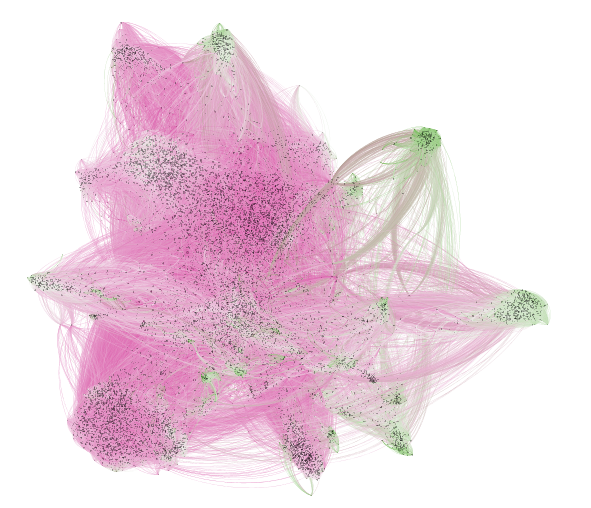
\includegraphics[scale=.45]{figs/megarrede}
\caption{An example visualization of a mega network with tenths of thousands of participants derived from Facebook ego networks.
	For further information please see Section~\ref{sec:megarrede}}.
\label{fig:megarrede}
\begin{flushleft}\footnotesize
Source: By the author.\
\end{flushleft}
\end{center}
\end{figure}
% arte pelo Pedro Paulo Rocha

\section{Social structures live streaming (networks and language-related)}\label{sec:sss}
A strong trait I could observe with the cycles of information gathering and diffusion (see Section~\ref{sec:colDif})
is the timid appropriation of the social structures by their participants.
Some people are enchanted by the figures,
others by the concepts and by the perception of the social aspect of themselves,
sometimes called ``network being'' or `` I-network '' by interested parties during the broadcasts.
In these contexts, academic theories, such as the Network Actor Theory (Latour),
were rarely recalled directly, even by specialists.
The efficiency of the intuitive discourse to communicate about these interests is remarkable.
The impulse to report the impressions resembles the urge to report dreams,
with glimpses of subtle and unconscious structures and sequential forgetfulness.
In this context, in order to spread about how our traces can be observed and taken advantage of,
we programmed screens of social structures streaming in HTML pages.
Only Twitter was used, and networks yield by retweets,vocabulary and hashtags were contemplated.
The screens could also display recent tweets, more occurring words, co-occurrences,
and other simple text information.
These screens were used e.g. in the Arena NET Mundial event
and in mobilizations such as the one identified with the \#ocupaGOV hashtag.
Figures~\ref{fig:telao1} and~\ref{fig:telao2} exemplify such interfaces.
They were updated live as tweets were sent by all Twitter users whose messages
contained the selected hashtags.
The source code is publicly available in~\cite{teloes} and uses Meteor and D3.js as frontend and
Python behind the scenes for streaming tweets and deriving network structures and measures.

\begin{figure}[H]
  \centering
    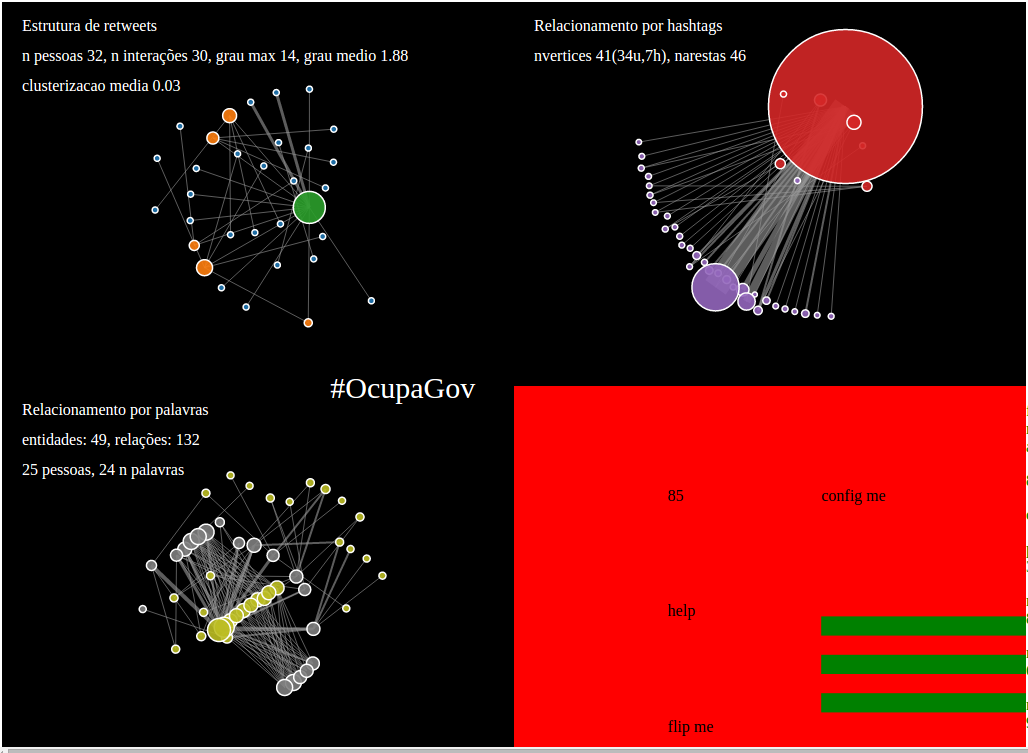
\includegraphics[width=.85\textwidth]{figs/telao1.png}
  \caption{Network interfaces of the live social structures streaming gadgets we programmed.
	Further information is on Section~\ref{sec:sss}.}\label{fig:telao1}
\begin{flushleft}\footnotesize
Source: By the author.\
\end{flushleft}
\end{figure}

\begin{figure}[H]
  \centering
    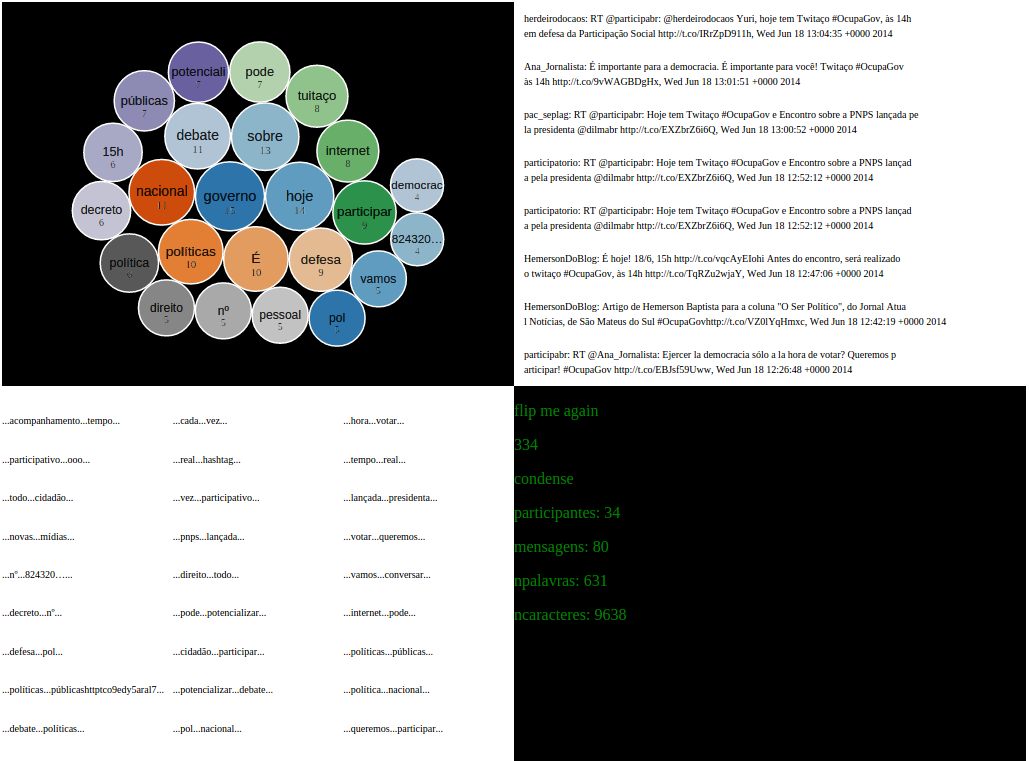
\includegraphics[width=.85\textwidth]{figs/telao2.png}
  \caption{Language-related interfaces of the live social structures streaming gadgets we programmed.
	Further information is on Section~\ref{sec:sss}.}\label{fig:telao2}
\begin{flushleft}\footnotesize
Source: By the author.\
\end{flushleft}
\end{figure}

\section{Ubiquity of inequality: a simple model that explains why power laws are so frequently found in empirical data}
	Inequality has always been a crucial issue for human kind, particularly concerning the highly unequal distribution of wealth, which is at the root of major problems facing humanity, including extreme poverty and wars.
	A quantitative observation of inequality has become commonplace in recent years
	with the expanding recognition that many natural and man-made systems can be represented as scale-free networks,
	whose distribution of connectivity obeys a power law.
	These networks may be generated by the preferential attachment for the nodes, within the so-called rich-gets-richer paradigm.
	In~\cite{ubiIne} we introduce a simple model that explains the ubiquity of inequality, based on three simple assumptions applied to a generic system with numerous parts.
	The first assumption is the diversity of the components.
	The second assumption is a uniform distribution of resources for individual components.
	The third assumption is that the amount of each resource input to the system is fixed.
	This implies that the more resources are allocated per component, the less numerous are such components,
	with the conservation of the amount of resources distributed through $component\; wealth = \frac{resources}{component}$.
	The second and third assumptions are conservation laws: energy is conserved through each resource and through component wealth.
	This can be geometrically described by the distribution of object sizes in an n-dimensional Euclidean space.
	Applying these assumptions to a generic system results in a power-law distribution, whose coefficient is the number of inputs that are independent from each other,
	i.e. the dimensionality of the allocated resources.
	Even though there is no restriction to the value of the coefficient,
	in practice we observe that existing systems normally exhibit a coefficient between 1.5 and 3.0.
	With our simple model it is not possible to determine whether this limitation in the coefficient values arises from a fundamental principle, but we indicate reasonable hypotheses.
	The assumptions in the model lead to a framework analogous to the laws of thermodynamics:
	conservation of resources and a time arrow pointing to inequality.
	Since these assumptions are easily justified based on established knowledge,
	the model proves unequivocally that inequality is ubiquitous.
	We also discuss ways to control this tendency to inequality,
	which is analogous to a decrease in entropy in a closed system induced by an external action.

\subsection{Three equanimous aspects of scale-free networks}
The model presented in last section exposes an equanimous aspect of power laws:
the resources are uniformly distributed along the concentration of resources.
In considering complex networks, there are two other aspects which are also equanimous:
the components (vertices) participate in many networks and potentially have different concentrations
of resources in them; the components changes their amounts of resources as the network evolves.
This is particularly interesting as it is countercurrent regarding the present-day hubs boast
in scale-free networks theory.
Furthermore, we also sustain in Section~\ref{sec:impl} that the intermediary vertices are both more relevant for the
network structure and are more likely to be authorities in human social networks.
There is a sketch of an article dedicated to these issues in~\cite{eqFree}.

\section{Systematic measurements related to the two-sample Kolmogorov-Smirnov test}
The two-sample Kolmogorov-Smirnov test relates the number of samples and the Kolmogorov-Smirnov statistic
to a confidence level in rejecting the null hypothesis (that the underlying distributions of the samples are the same).
However, if sample sizes are large enough, the test rejects the null hypothesis even with arbitrarily small differences
in the distributions.
In terms of Section~\ref{sec:ks}, $c'$ can be arbitrarily large for any non-zero value of
$D_{n,n'}=sup_x[F_{1,n}-F_{2,n'}]$
if the sample sizes $n$ and $n'$ are large enough.
As a way to better grasp these relations between 
$c'$,
$D_{n,n'}$,
$n$ and $n'$, we made systematic measurements using many distributions
(normal, uniform, Weibull, power) and different parametrizations.
These measurements are presented in~\cite{kolmSmir}.

\section{The Algorithmic Autoregulation (AA) software development methodology}\label{sec:aa}
In~\cite{aaPaper} we present a new self-regulating methodology for coordinating distributed team work called Algorithmic Autoregulation (AA),
based on recent social networking concepts and individual merit.
Team members take on an egalitarian role, and stay voluntarily logged into so-called AA sessions for part of their time 
(e.g. 2 hours per day), during which they create periodical logs - short text sentences - 
they wish to share about their activity with the team.
These logs are publicly aggregated in a website and are peer-validated after the end of a session,
as in code review. 
A short screencast is ideally recorded at the end of each session to make AA logs more understandable.
This methodology has shown to be well-suited for increasing the efficiency of distributed teams working on 
Global Software Development (GSD), as observed in our reported experience in actual real-world situations.
This efficiency boost is mainly achieved through 1) built-in asynchronous on-demand communication in 
conjunction with documentation of work, products, and processes, and 2) reduced need for central management,
meetings or time-consuming reports.
Hence, the AA methodology legitimizes and facilitates the activities of a distributed software team.
It thus enables other entities to have a solid means to fund these activities, 
allowing for new and concrete business models to emerge for very distributed software development. 
AA has been proposed, at its core, as a way of sustaining self-replicating hacker initiatives.
These claims are discussed in a real case-study of running a distributed free software hacker team called Lab Macambira.
This work was important for maturing concepts related to social networks and thus contributed to the presented thesis.

\subsection{Essay on AA: detailing language and activity of a social networking platform}
While AA was important for some documents presented in this thesis~\cite{aaPaper,losd},
it played a central role in the first steps for analyzing social networks.
In the scripts and essay in~\cite{ensaaio} we started doing measurements of activity along time (e.g. days of the week),
of most incident words and of users just like we presented in the Methods and Results of this thesis.
The essay also discloses the AA implementations and conceptualizations.

\section{Social participation (OWL) ontologies}\label{sec:spont}
As a way to integrate participatory mechanisms, some OWL ontologies were developed within our research.
All the ontologies presented in the next sections have graph figures in the documentation for easing the use of
the conceptualizations.
In them, each node is a concept (an OWL class) and the directed edges correspond either to a taxonomic relation
(hypernymity, i.e. ``OWL class $\rightarrow$ superclass'' relation) or to another type of relation between concepts (i.e. OWL property).

\subsection{OPS: the Social Participation (OWL) ontology}
Participatory democracy advances in virtually all governments and especially in South America which presents a mixed culture and social predisposition.
 In 2012, civil, academic and governmental parties started elaborating the ``Social Participation Common Vocabulary'' (\vcps\ from the Brazilian name \emph{Vocabul\'ario Comum de Participa\c{c}\~ao Social}), as a public and online process. By May 2013, first reference documents were publicized, together with preliminary \owl\ code, logos, and a diagram for a general ``public consultation''.
The \corais\ platform kept online records of the process, like discussions and text drafts. 
The article~\cite{ops} presents this material and proposes, based on it, the ``Social Participation Ontology'' (\ops\ from the Brazilian name \emph{Ontologia de Participa\c{c}\~ao Social}). To create  this new ontology, these steps were followed: correction of ontological contradictions and \owl\ errors in \vcps; inclusion of concepts documented in the \corais\ platform (but not present in \vcps) in a preliminary version of \ops; entity name standardization; translation of labels to Portuguese, Spanish and English; an ontology expansion; creation of linked data examples and  a \sparql\ endpoint; compilation of use cases from researchers and public managers. Ongoing work involves further adoption of \ops\ by the official Brazilian federal portal for social participation and  NGOs, and linkage to other ontologies for participation. The \ops\ is being used as an upper ontology, and all classes linked further to \foaf\ and \bfo\ as higher upper ontologies.

\subsection{OPa: the ParticipaBR federal social participation web portal (OWL) ontology}\label{sec:opa}
There were two very distinct ontologies for the ParticipaBR Brazilian federal social participation web portal.
The first ontology, centered around the concepts of Portal, Participant, Community and Participation Mechanism,
was conceptualized by the community by idealizations of what a
federal social participation portal should be and the main documentation is available in~\cite{opa0}.
The second ontology was derived from the data of the portal and is available in~\cite{opa}.
The first ontology was interesting for the specialists and might help in creating new web portals but did not fit
ParticipaBR data: ontology classes and properties did not find correspondent entries while
ParticipaBR items did not have correspondent structures in the ontology.
Therefore the second ontology was created.

\subsection{OntologiAA: the AA (OWL) ontology}\label{sec:ontologiaa}
An ontology for the AA mechanism described in Section~\ref{sec:aa} was developed and is documented in~\cite{opa}.
This ontology is depicted in Figure~\ref{fig:aaOn}.
\begin{figure}[h!]
\begin{center}
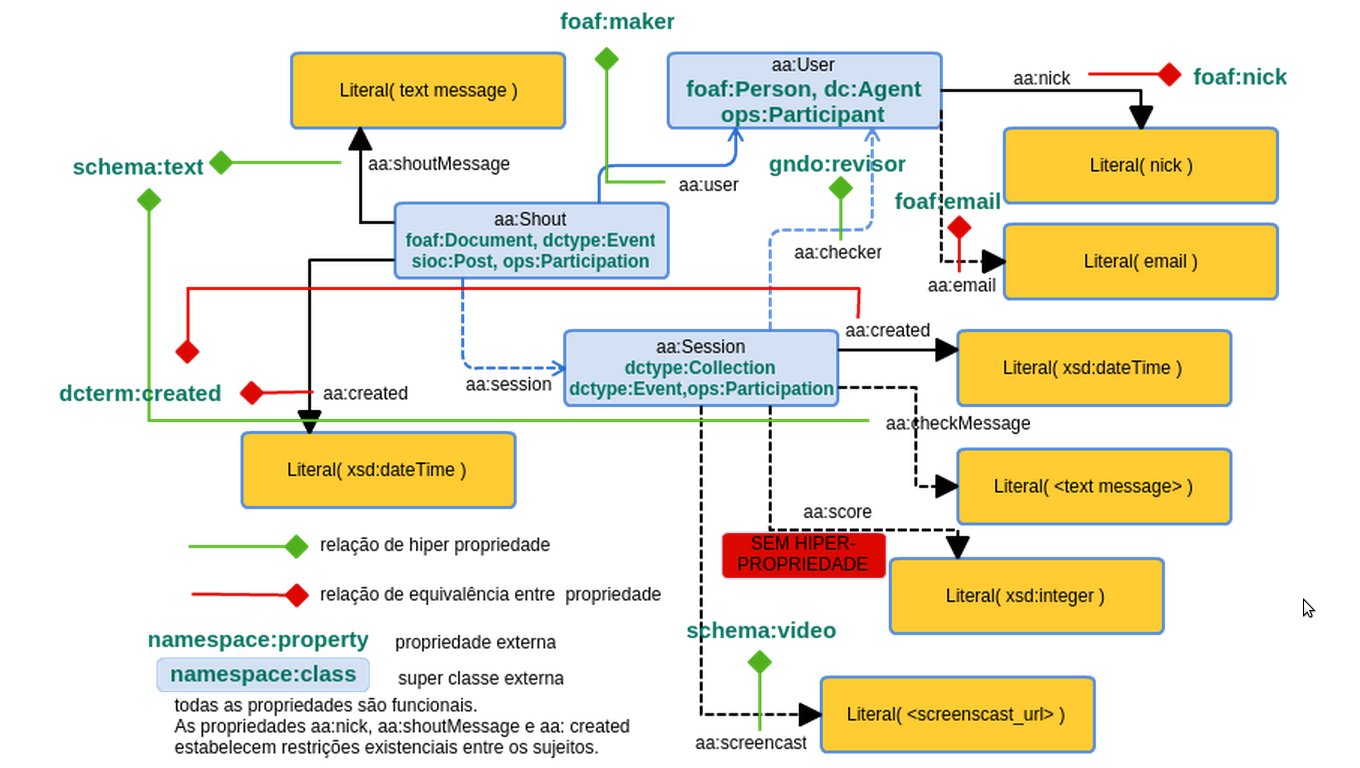
\includegraphics[scale=.3]{figs/ontologiaa}
\caption{A pictorial representation of the AA Ontology.
	For further information please see Section~\ref{sec:ontologiaa}}
\label{fig:aaOn}
\begin{flushleft}\footnotesize
Source: By the author.\
\end{flushleft}
\end{center}
\end{figure}

\subsection{OCD: Cidade Democrática (OWL) ontology}
An ontology for the Cidade Democrática civil social participation platform was developed and is documented in~\cite{opa,ocd}.
For this ontology we developed the first version of the data driven ontology synthesis method presented in Section~\ref{sec:ontSyn}
and that was used for obtaining the second ParticipaBR ontology described in Section~\ref{sec:opa}.

\subsection{Social Library: conference, forum, council, ombudsman, public consultation, dialogue table, decree 8.243 and IPEA}
The OBS (Social Library Ontology, from the Portuguese ``Ontologia da Biblioteca Social)
and the VBS (Social Library Vocabulary, from the Portuguese ``Vocabulário da Biblioteca Social)
were derived from two types of sources: specialists (political authorities)
and the decree 8.243 that organized the Brazilian social participation instances.
The specialists contributed in two manners: by means of a Workshop given by the author 
of this thesis in the Presidency Palace in Oct/20/2014
and by means of dedicated interviews.
Social participation instances and mechanisms were systematized and general
social participation conceptualizations given separately by the Brazilian Presidency
and the IPEA (Institute for Applied Economic Research).
Core documentation is in~\cite{opa,vocabP}.

\subsection{An (OWL) ontology for the Magic Box (Caixa Mágica)}\label{sec:mb}
The Magic Box was conceived in LabicBR as a way to enhance social participation
in micro territories through WiFi.
Core contributors are Ricardo Augusto Poppi Martins (Brazil), Marco Konopacki (Brazil),
Mariel Zasso (Brazil), Renato Fabbri (Brazil), Erick Berssaín García Ventura (Mexico),
Ana Karen Moreno Ramos (Mexico), Norma Ruiz (Mexico),
Thomaz Anderson Barbosa da Silva (Brazil), Luis Astorquiza (Colombia) and Carlos Espinosa Llerena (Ecuador).
I formalized in OWL the ontological conceptualization of the Magic Box and keep it available at~\cite{caixamagica}.

\section{Triplification routines of relational data into RDF}
All the ontolgies reported in Section~\ref{sec:spont} have \emph{triplification}
routines which translate (relational and non-relational) data to RDF.
The only exception is OBS which does not directly relate to data in any platform
but to knowledge yield by specialists.

\section{Ontology of the Work}
The Ontology of the Work (OT from Portuguese ``Ontologia do Trabalho'')
is a conceptualization formalized in OWL of the knowledge involved in this thesis.
It was used in the qualification of the doctorate and is available at~\cite{OT}.
The ontology is quite useful for grasping the purpose and knowledge fields related to
the research but is too large for including here a meaningful image.

\section{ORe: Ontology of the Research and data records}
This is a rather experimental development aimed at keeping track
of the research process.
Most importantly, in~\cite{ore} are a hook for registering new entries
very similar to what is done through AA (see Section~\ref{sec:aa}), and a script and resulting RDF file
with research notes.

\section{Genesis of this research: complex social networks analysis by emails}
The first written systematization of our findings among networks derived from email lists
is~\cite{comp1}.
It was important for a several reasons: we confirmed the scale-free outline of the connectivity distribution
in these networks;
we first observed the asymmetry of edges;
the article invoked disrupting discussion in email lists and private messaging, specially at the Metareciclagem email list.
This work received collaborations of Vilson Vieira da Silva Junior, Lucas da Silva Oliveira
and Prof. Dr. Ricardo Fabbri (IPRJ/UERJ)
and was presented in the XVI Meeting for Computational Modeling.

\section{United Nations Development Program consulting}\label{sec:undp}
In the year of 2014 this research was endorsed by the United Nations Development Program
with a consulting contract (2013/00056, project BRA/12/018).
The collaboration was centered around complex networks,
natural language processing/text mining, linked data and social participation,
all of which are approached in the introductory Chapter~\ref{ch:int}.

\subsection{Partnership with the Brazilian Presidency}
This consulting was proposed as a partnership between me
and the Brazilian Presidency.
Many of our meetings and immersions were held by the Brazilian Palace (\emph{Palácio do Planalto})
and I could learn deeply by working with specialists and authorities.
Among the most important of these meetings I should point
my participation in the \#arenaNetmundial virtual hub for the NET Mundial world meeting (Apr/2014)
and an internal Workshop I headed in the presidency (Oct/2014) with many State leaders experienced with social participation.
The supervisor was Ricardo Poppi (with contributions by Ronald Emerson Scherolt da Costa)
who was then the presidential general coordinator of new media.
More names of people involved in this collaboration are on the Acknowledgments in the beginning of this thesis.

\subsection{Description of each product}
It was assignment to attend to meetings and to generate 5 products:
\begin{itemize}
	\item Product 1: the first ParticipaBR ontology~\cite{opa0}.
	\item Product 2: context, triplification of data, example of usage~\cite{pnud2}.
	\item Product 3: resources classification and recommendation~\cite{pnud3}.
	\item Product 4: proposals of enhancements for the ParticipaBR portal~\cite{pnud4}.
	\item Product 5: integration of ParticipaBR and other participation instances~\cite{opa}.
\end{itemize}

I also presented further documents:
\begin{itemize}
	\item Extra product: notes on reading products of other consultants~\cite{pnudExtra}.
	\item Extra product: an essay on the endeavor of using complex networks, text mining and linked data for social participation~\cite{ensaio}.
	\item Extra document: specification of software and hardware requirements for a monitoring system. Presented in the next section.
\end{itemize}

\subsubsection{Infrastructure of a monitoring system for social participation}\label{sec:monitoring}
In contributing with the presidency we found the need for a monitoring system of social networks
which could be used by the civil society.
This was thought about in terms of linked data with a SparQL endpoint, streaming of tweets and data processing through Python
and a Javascript frontend with Meteor and D3.js.
The resulting document with the demand~\cite{sm} also presented hardware and operational system issues
and circulated among consultants and employees of the National Secretariat of Social Articulation (SNAS) and 
the presidential board of information technology DITEC (``Diretoria de Tecnologia da Informação da Secretaria de Administração da Casa Civil da Presidência da República'').

\section{Contributions to the National Plan and Commitment for Social Participation (PNPS and CNPS) related to the Decree 8.243}
I made substantial contributions for the public discussion regarding these Brazilian social participation
endeavors.
More specifically, I commented each of the items in the public discussion platform~\cite{participaPNPS},
and made some scripts~\cite{analisePNPS,pcPS} for analyzing the Decree and commitment declaration and the social networks considering these issues.
There is also a document with further analysis of these documents and social participation instances in~\cite{lmPS}.

\section{Meetings at the Ministry of Education (MEC)}
I was asked to join at least two meetings at the Brazilian Ministry of Education (MEC)
at the genesis of this research.
These are probably the first occasions where I presented the possibility of using
complex networks and text mining (at then more focused in natural language processing)
for social participation.
These were also where we first thought about linked data/semantic web to enable a
Brazilian social participation cloud and a better organization of our data.
We had our efforts directed towards strengthening the online trends of CONAE (National Education Conferences).
I learned and contributed with the authorities and specialists present at the meetings,
specially Ricardo Poppi, Arlindo Cavalcanti Queiroz and José Ivan Mayer de Aquino.

\section{Other non-academic events attended: LabicBR, I Technological Week of Ubatuba, Regulatory Landmark of Civil Society Organizations (MROS), Social Participation National Plan (PNPS) Forum}
There were many non-academic meetings attended to in the course of this research,
some of them mentioned in Sections~\ref{sec:undp},~\ref{sec:soundSkull} and~\ref{sec:serv}.
Other events I attended to that are not mentioned are the I Technological Week of Ubatuba, where
we assisted programmers and presented and interface and a performance in livecoding using Vivace (see Section~\ref{sec:vivace}).
Another important event was the LabicBR (the Brazilian edition of the ``Laboratorio iberoamericano de Innovación Ciudadana'')
where I joined an international team and developed the Magic Box ontology (see Section~\ref{sec:mb}) and a data visualization interface
with PHP, Javascript and D3.js.
At MROSC hackaton, I developed an online network visualization for data related to civil organizations~\cite{oscEmRede} using
Meteor, D3.js and Python.
At the PNPS intercouncil forum I had the opportunity to debate with activists and authorities about enhancing social participation
through virtual means and program a minimal gadget through which the society could vote using Twitter~\cite{votoTwitter}.
By browsing through documentations I also found other events which were relevant for this research,
such as the
Dialogues Governance and Society: new forms of social participation in the policy
(``Diálogos Governo e Sociedade: novas formas de participação social na política''),
an event held by the presidency in Jul/18/2013 in the presidential Palace,
and my contribution as an advisor and speaker at the Hackaton held by the Rio de Janeiro Art Museum (MAR)
and SESI at Oct/13-15/2015 where I also developed a linked data representation and OWL ontology of data from MAR collection~\cite{hackmar}.
All attendances should be in my Lattes curriculum page~\cite{myLattes} in near future as
I need them formalized for academic purposes, specially when finishing this doctorate.
In all these contributions, my traveling and subsistence expenses were paid by the organizers who invited me.

\section{Academic events attended: critical theory, complex systems and a text mining workshop}\label{ap:anphy}
There were three academic conferences
which were most important for presenting the background and preliminary results to the scientific community
and to advance conceptualizations related to researching human social structures.
Two of these were Brazilian conferences~\cite{50uni,IICri} of the Nexos research network related to philosophy and social psychology
and the other was an online presentation~\cite{ccs15} on the Conference on Complex Systems CS-DC'15
(Complex Systems Digital Campus ’15 – World e-Conference).
Of some relevance was attending to the Seminar on Open Knowledge in the University
(Seminário sobre o Conhecimento Aberto na Universidade) at UFPA
in which I held a data mining workshop and took part in a discussion table about open academic knowledge.
I also presented some developments at two internal IFSC/USP conferences (SIFSC).
For enhancing my familiarity with research in linguistics from the computational standpoint,
I attended to all presentations on the EILIN 2013 (Winter School on Formal Linguistics)
but did not present any of our research.

\section{Govern art}\label{sec:govArt}
Many of the developments presented in this thesis were accompanied by the construction of online gadgets
and some of them were artistic.
As we labored with government parties and issues,
the concept of ``government art'' emerged.
The proposal is to make art with government/State symbols.
Some of the realized examples of govern art are in~\cite{aars}.
The Meteor company unfortunately stopped their free services which
allowed these gadgets to keep functioning online.
The Figure~\ref{fig:gart} exemplifies a Govern Art instance.

\begin{figure}[h!]
\begin{center}
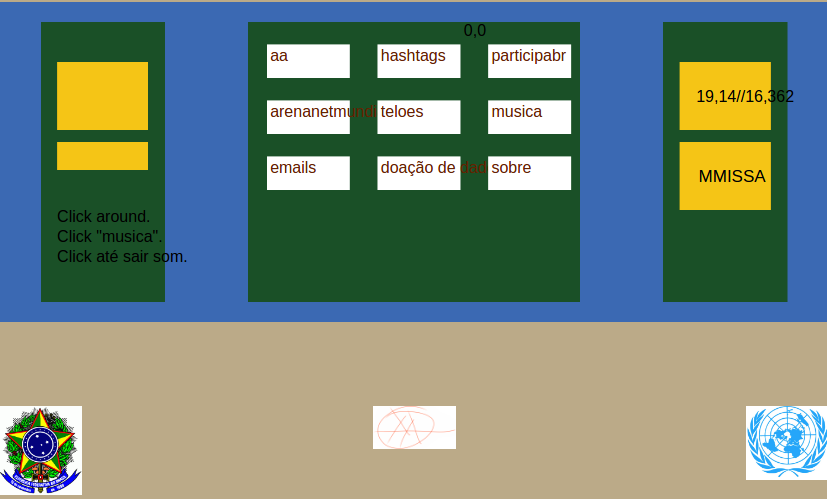
\includegraphics[scale=.45]{figs/govArt}
\caption{An example of a Govern Art instance with the emblems of the Brazilian presidency and the United Nations.
	This webpage had also the emblem of the labMacambira.sf.net and could display animated networks and play music by mapping network structures to sound.
	Also, the page had special widgets which, if clicked, would change the colors and layout and individual widgets.
	For further information please see Section~\ref{sec:govArt}.}
\label{fig:gart}
\begin{flushleft}\footnotesize
Source: By the author.\
\end{flushleft}
\end{center}
\end{figure}
\section{Sounding Skull: a Rilke proposed transcendental experiment}\label{sec:soundSkull}
Rainer Maria Rilke proposed transdisciplinary experiments involving attempts to hear the
sounds of the grooves in the cranium~\cite{rilke}.
We created a performance group to make such experiments.
This was important for our research as an interface
by means of which different backgrounds could be exchanged by the participants.
The performers of the Sounding Skull group are:
Prof. Dr. Massimo Canevacci, Prof. Dr. Marília Pisani,
Rita Wu, Caleb Mascarenhas Luporini and Renato Fabbri.
There were also occasional but important participation
by Juliana de Souza, Gulherme Lunhani and Vilson Vieira.
Most important presentations were in the AVLAB 6 (an event about art, media and politics)
and in closing the International Critical Theory Conference of Rome (online participation).

\section{Ideal ideas: a physical modeling of the mind}
Thought can be conceived as constituted by ideas.
Ideas can be conceived in a way that any set of ideas is an idea.
In~\cite{idealIdeas} we present a physical and formal description of the
thought in such conceptualization.

\section{Webpages}
% ARS, texto para pedro, MMISSA, MyNSA
There were many webpages produced by this research.
Maybe the most important of them are the ones directly related
to Social Network Analysis and the endeavors for collection and diffusion of information~\cite{sfARS,rfARS}.
One interesting instance is the online publication of the text ``Cognitive clouds and the unification of humanity''~\cite{nuvens}
by the Cyberium transmedia collective and the Nós Digitais digital cultural pole.
Some pages are not online anymore, such as the ones referred to in Sections~\ref{sec:govArt} and~\ref{sec:sss},
mainly because free services were withdrawn.
All texts and software developed in this research are available in online pages,
most often hosted by Github and arXiv but also in Wikis, Sourceforge and independent instances.
A simple but useful example of a gadget used by means of a webpage that
stood the test of time is an AA interface~\cite{aaclient} for displaying the shouts
(see Section~\ref{sec:aa}).
A minimal homepage made for sharing ongoings related to this research is~\cite{ttmio}.

\section{Collection and diffusion of information in social networks}\label{sec:colDif}
In realizing the initial proposal of this research of enabling the participants to take action
in their networks by means of scientific knowledge, it was considered central
to tackle the collection and diffusion of information.
This was achieved in a number of ways which are documented in this thesis and bibliography items.
We next expose four main practices we developed which are not documented elsewhere.

\subsection{Progressive network activation from peripherals to hubs for a crowdfunding}
This is maybe the most powerful mechanism by which we performed collection and diffusion of information.
The results were very effective in spreading information about social networks,
in gathering knowledge from diverse parties and in modifying the social structures
in which I participate.
Most concretely, academics came to São Carlos for formal meetings,
new collaborations were established (such as the UNDP consultating described in Section~\ref{sec:undp}),
money was obtained (various contributors transferred a total of about 3000 Brazilian reais)
and my Facebook network increased about 50\% with individuals interested in the research.
The process consisted in:
\begin{enumerate}
	\item Downloading my Facebook friendship network. This was done by means of the Netvizz software,
		which is not possible nowadays and requires scrapping of Facebook pages because of new usage terms.
	\item Sorting my friends from the less connected to the more connected, i.e. from my friends that have less friends in common with me to the ones that have more friends in common; i.e. from periphery to hubs.
	\item Sending private messages for each of my friends, in such order.
		The messages were derived from a template I conceived in which I exposed the research and the information diffusion process.
	\item Making steps 1-3 for three times.
\end{enumerate}
In each cycle of steps 1-3, my friendship network grew about 15\% and there were typical reactions in each cycle.
In the first cycle, my Facebook contacts reacted with estrangement and replies such as ``what are these network structures?'',
``what are you doing? I can't understand!'', ``I never though of such a thing as these networks''.
In the second cycle, they replied with interest and support.
In the third cycle, they were establishing collaborations with visits, elaboration of documents and technologies and
co-working proposals.

The main problem of these results is that they are not still confirmed by performing the experiment again.
Even so, the data related to performing these three cycles can be organized by downloading my personal data in the Facebook interface.
Given that the diffusion process was done in Dec/2012-Jan/2013, it was frequently thought of by fellow specialists as
having some influence in the civil society mobilization that occurred in Brazil in Mar/2013 and thereafter.
A very simple PDF document was built afterwards for delivering back these results to the networks~\cite{docDif}.

\subsection{Instantaneous network activation by betweenness and closeness centralities}
This was first thought in meetings with the artist and activist Pedro Paulo Rocha.
The idea was to activate the network not by means of a longstanding process such
as described in the last section, but by an ephemeral endeavor.
There were some artistic performances with this proposal, in which I did
not participate.
Nevertheless, there was one of these instantaneous activation processes that
I have done in conjunction with other specialists which was rather interesting.
In analyzing Facebook ego friendship networks, the set of $\approx 50$ members with
the greatest betweenness centrality was disjoint with the set of $\approx 50$ members
with the greatest closeness centrality, which is very unexpected.
Therefore I proposed that one should send the same message to both set of friends separately.
The messages were different for each person performing the experiment,
and it was about something they were interested in and wanted to spread and get feedback.
The result was systematic: the set of friends with greatest betweenness always reacted very friendly
with encouraging messages and sharing the original message in their timelines.
The set of friends with greatest closeness always reacted with many leaving the chat group
and with no replies.
We hypothesize that these reactions are because the large betweenness set of friends is more
likely to have control over the information flowing in the corresponding ego network while
the large closeness set of friends is more likely to observe/receive influence by the information.

This experiment was performed by partners related to the consulting reported in Section~\ref{sec:undp}
and other partners involved in making an international technoshamanic festival.

\subsection{Massive tagging in Facebook and email crossposting}
One very simple process by which we performed collection and diffusion of information
was by tagging many friends in Facebook posts.
Currently, one can tag up to 99 friends in a post
and we did not find any limit for tagging friends in comments.
If one makes abusive use of tagging (too many posts or too many comments)
the Facebook platform sometimes restricts the permissions of that user.
Even so, I have made many posts with up to 99 friends tagged and tagged more
friends in the comments and made experiments such as the ones described in the
last sections and never got restricted.
It seems that the platform has some automated behavior but employees actually
perform the restrictions at least in some cases.
The employees might check the posts, tagging and messages to see if it is
really spam or in anyway abusive.
In~\cite{anExp} are some notes and data of one of these experiments (and a preliminary script for analysis).

Another powerful way by which I many times performed diffusion and collection
of information is by crossposting, i.e. by sending a message to many email lists
at the same time.
I find this very effective but the email list users often report such practice
as abusive.
Even so, no one has ever sent me a message reporting discomfort with my crossposts.
There was one occasion some years ago when a user replied with a challenge for
arguing why the crosspost what appropriate and then made some good contributions.
I personally perceive that this prejudice against crosspost is one of the main reasons
why email groups are losing users to other communication protocols such as Facebook, Whatsapp, Telegram and Diaspora.

\subsection{SERVDDCR online video conferences}\label{sec:serv}
Video conferences has been a major practice in reaching other interested parties.
Of the many video conferences performed in this research,
the SERVDDCR might be the most interesting.
These were monthly online meetings publicly announced, broadcasted and
recorded and kept available online (at Youtube) with other documentation produced.
The conference was often full (the Hangout Onair interface reached the limit of connections)
and participants had diverse background, ranging from arts and politics to physics and philosophy.
SERVDDCR means Society and State in Virtual Meeting for Direct or Connective Democracy or Gathering
from the Portuguese ``Sociedade e Estado em Reunião Virtual para Democracia Direta ou Conectiva ou Rolezinho'').
SERVDDCR is leet for Portuguese ``servidor'' (server).
Most documentation should be found in the Facebook group SERVDDCR~\cite{servidor}.

\section{Anthropological physics}
The study of complex systems can be undertaken as a physics endeavor,
specially if complex networks and statistics are into play. When the complex
system is constituted by people, intriguing questions arise from diverse field such as math, ethics, and sociology. The “anthropological physics”is an approach to these scenarios that enables scientific research while resolving ethical and moral issues by an open study of the self.
	It yields a transdisciplinary practice whose relevance emanate from anthropological
and physical matters, from human constituted systems and natural laws.
A sweet spot was found in recent civil, government and academic efforts~\cite{opa,ensaio}, and has been called anthropological physics. General characteristics are:
\begin{itemize}
	\item Exposure of the researcher to the environment of interest, such as virtual social networks.
	\item Use of the annotations from the exposure, be them activity logs, friendship or interaction networks, textual contents, etc.
	\item Upon need, expansion of observations to encompass open datasets or data donated by partners.
	\item Observance of natural laws as they appear in network structures and natural language.
	\item All resources are kept as open and publicized as possible, including software, data, and writings.
\end{itemize}                                                                                                                                     
A short report on the first insights regarding anthropological physics is on~\cite{anPhy}.
Further notes on a public discussion about the anthropological physics concept are on~\cite{anPhy2}.
A significant stimulus for the participation in the academic events described in Section~\ref{ap:anphy}
was the maturing of this topic.

\section{Bots used in labMacambira.sourceforge.net}
There has been many bots (software chat agents) used in labMacambira.sf.net.
They were relevant for our research in linguistic experiments and were used
for developing software, social articulation and for recreational purposes.
In~\cite{trabBots} we present the most relevant of these bots together with
brief words on labMacambira.sf.net and notes on past and future plans on using
these chat agents.

\section{The Python Natural Language Toolkit (NLTK) short introduction}
When we started this research, the documentation of NLTK was either lengthy or
scattered.
Therefore, we understood useful to make a very short introduction to NLTK
exemplifying the most frequent uses such as tokenization, stemming, lemmatization and
part-of-speech tagging in both English and Portuguese.
We also provided ideas for researching social networks which followed directly from
these basic tasks.
The document is at~\cite{trabNLTK}.


\section{OvO: Ouvir para Olhar (hear to see)}
These meetings were headed by Prof. Dr. Michel Hospital (DEE/UFSCar)
with the purpose of maturing audiovisual research.
The most important of these were: a meeting at DEE/UFSCar for discussing research with Prof. Dr. Emerson;
a meeting at the Sérgio Mascarenhas auditorium (IFSC/USP) with researchers from DEE and the UFSCar Psychology department
for exposing research ongoings where I presented about audio and music, Vilson Vieira presented about imaging processing
and Prof. Dr. Michel Hospital presented about OvO;
a workshop in Apr/13/2015 about audio and music I held at an IFSC/USP computer laboratory.
A proposal of Prof. Dr. Hospital for which we dedicated some attention was the
mapping of visuals for sound for accessibility.
Some scripts and documentation are found in~\cite{ovo} and links therein,
including some very simple mappings of networks features to musical sounds.

\section{Complex networks \emph{gradus ad Parnassum}}
\emph{Gradus ad Parnassum} is a type of document that contains a gradual progress for grasping a subject.
We sough about a \emph{gradus} for complex networks for some years and the outline is:
basic notions and network models such as presented in Section~\ref{ch:int};
notes in network stability and linguistic differentiation as presented in this thesis, but in simpler form;
methods and tools for harnessing the networks of the participant, which includes what is presented in Section~\ref{sec:colDif};
a report of using this framework.
Although the document might be of academic interest,
Geraldo Magela de Castro Rocha agreed on doing an artistic publication by independent means
with the purpose of spreading the knowledge in the general civil society.
A very incipient sketch of the document is at~\cite{gradus}
with a small script relating mythology and networks.

\section{Graph-based semi-supervised learning}
I made software implementations of two graph-based semi-supervised learning algorithms
(i.e. supervised learning algorithms that make use of unlabeled data):
``mean-cut'' and ``label propagation''.
These were particularly important in 1) obtaining better classification results
than with supervised learning algorithms for distinguishing between positive
and negative sentiments in speech samples; 2) maturing my reasoning about graphs
and learning algorithms, specially grasping the power semi-supervised algorithms.
These implementations are available in~\cite{ssl} with documentation.

\section{Microtales}
These are artistic small texts~\cite{microcontos}.
Both poems and tales are incident.
They are important for registering ideas and viewpoints
and because I used them in some diffusion and collection of information experiments
(see Section~\ref{sec:colDif}).

\section{Pingo game sound effects}
Pingo is a Tamagotchi-like experimental game for adults
developed by Edson de Oliveira Correa Jr. and Prof. Dr. Ricardo Fabbri (IPRJ/UERJ).
I made a sound effects bank for the game which is available in~\cite{pingo}.
It was the only oportunity I had to dwelve into gamification in this research.
Two of the most powerful approaches to making social participation and
these complex networks, text mining and linked data more interesting for the
user is gamification and audiovizualization of data.

\section{Textual analysis of dreams for schizoanalysis and art}
The psychologist Dr. Fabiane M. Borges proposed to me the analysis of dreams through text mining
with the goal of using the results in a schizoanalysis course.
We obtained interesting results and poems which were used in
the third module of the schizoanalysis course (held at Rio de Janeiro,
Nuvem house, Oct/17/2015).
Scripts and documentation are at~\cite{sonhos}.
We intended to make further analysis by including more dreams.
The texts describing the dreams were sent to me, but I was not able to dedicate time
as needed and we agreed to do these analyzes in a book or
as we understand fit in the future.

\section{Toki Pona language incursions}
In advancing with the studies of language for this research,
I found the need to learn a conlang (i.e. a constructed language).
Candidate languages were Esperanto, Lojban and Toki Pona.
The last of these was chosen for being very minimalist,
with only 14 phonemes and 120 words,
and presenting a different standpoint to language usage
(I am fluent in English and Portuguese and have basic skills in German).
I present some contributions for the Toki Pona language in~\cite{tokiio}
and some scripts for exploring the structure of the language and for
a Vim syntax highlighting in~\cite{tokir}.
% artigos
% vivace and freakcoding

\section{Vivace: a collective livecoding interface}\label{sec:vivace}
Livecoding is a creative and performing technique in which the
presenters write source code in real time which controls audiovisuals.
Often a livecoding session is done by projecting the code being written in
large screens (such as by the usage of a datashow) as a way to yield
interest in a computer-based performance.
The performers on a computer is often though of as not as interesting
for the spectators as the performers on traditional instruments such as a piano or a guitar.
For the purpose of livecoding, Vilson Vieira wrote the software Vivace.
This software runs on a browser (such as Firefox or Chromium)
and can be accessed by multiple livecoders at the same time,
enabling even the audience to change the code and thus the performance.
The Vivace code controls audio and video and is important for
this research because it is a social network experiment.
A dedicated article was written for Vivace~\cite{vivacecmj}
and the source code is at~\cite{vivacecode} with further documentation.

\subsection{Freakcoding: the origin of the first livecoding subgenre}
By rehearsing with Vivace we started to develop an aesthetic.
When Caleb Mascarenhas Luporini introduced videos with monsters,
and we used sounds from many sources,
the Freakcoding genre emerged.
It is the first livecoding subgenre we have reports about.
We presented Freakcoding in some events including an edition
of AVAV (``AudioVisual Ao Vivo'') at São Paulo.
The \emph{Freakcoding Manifesto} is online and received
an independent publication~\cite{freakManifesto}.

\subsection{The largest livecoding performance we know about}
This was the start of our developments in livecoding.
Many labMacambira.sf.net was at the stage while both mine and Vieira's computer screens
were projected in the fifth Festival Contato, in 2011 at São Carlos.
I was using Vim, Vieira was using Emacs and we both were using the ChucK
livecoding language.
Gilson Beck was at the sound diffusion table.
As far as we know, it was the livecoding session with the larger audience
that ever took place at the time.
It is relevant for the research in this thesis because it was
a social experiment to present art by projecting code and sound
and a social experiment to perform the livecoding with so many performers.

\section{The scientific literary style}
One of the greatest things I was able to achieve in this doctorate
is the enhancement of my English writing.
The book~\cite{chuLivro} was helpful, as were Coursera and edX courses,
but the most valuable practice was writing with my advisor Prof. Dr. Oliveira
and using English daily for reading, writing, watching videos and hearing audiobooks.
I have the ambition of writing an article about the scientific literary style
by exposing canons and trends and proposing extensions such as artistic uses
of the scientific style and minimal and maximal size possibilities.
A very preliminary sketch is on~\cite{sciStyle}.

\section{Relevant precursory texts: free media letter, Submidialogy and Counterculture}
From the knowledge I acquired by being a member of the judging committee for the second
free media award of the Brazilian Culture Ministry (which distributed about 4 million reais)
I wrote the free media letter~\cite{cartaML} with a needed systematization of what free media is.
Separately, I had texts published in the Counterculture~\cite{ccd} and Peixe Morto/Submidialogy~\cite{subMid} independent books.
These are relevant for the research on this thesis as being first culminations of deep interactions
I had with activists and cultural agents which contributed to my understandings of social structures
and information diffusion and collection processes.

\section{A note of precedence of the documents presented in this thesis}
% As there were many resources and endeavors related to this thesis,
% both to the main body of the text and to this appendix.
The main article from which this thesis derived is~\cite{stab},
where we present the stability (or invariance) we found in human social interaction networks.
The second most important work is~\cite{rcText}, because it is where we
first presented the linguistic differences related to the hubs, intermediary and hubs
Erd\"os sectors.
The third most important document for this thesis is~\cite{losd}, where we
describe the linked database of human social structures.
The last important article is~\cite{versinus}, in which we outline the Versinus method for visualization
of social networks by animations.
These contributions should be appreciated with their Supporting Information documents
where many measurements are presented and thus raises relevant evidences.
Main results from other efforts are listed in this appendix together with documents which
are relevant for~\cite{stab,rcText,losd,versinus}.

% Lattes:
% Mapa PtsSP
% https://www.escavador.com/sobre/4075206/renato-fabbri
\end{apendicesenv}
